\chapter{Results and Discussion}

This chapter discusses the analysis of the traffic and weather data. Moreover, this chapter will also discuss about the experiments performed and its results to evaluate the analysis of traffic and weather.

\section{Traffic and Weather Analysis}

\subsection{Weather Analysis}

\subsubsection{Seasonality}

In spite of having a daily pattern, however, there are weather variables whose pattern would not last for every day of the year or even a week. One of these weather variables is precipitation. In the autocorrelation of precipitation (see Figure \ref{figure_autocorr_precip}), it could be observed that despite having a daily seasonality, the pattern of the previous day cannot be barely used to predict the amount of precipitation to be expected today, as indicated by the weak correlation as it approaches its daily seasonality. Comparing it to the autocorrelation of temperature (see Figure \ref{figure_autocorr_temp}), the pattern of the previous day or even until a week ago can be used to predict the incoming temperature of the day, as indicated by the consistently strong correlation throughout the week.


\begin{figure}
  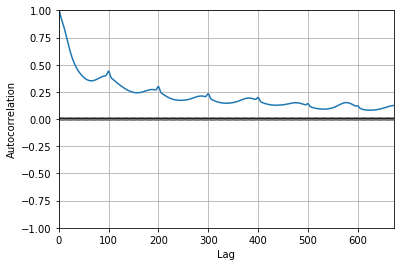
\includegraphics[width=\linewidth]
  {figures/figure_autocorr_precip.png}
  \caption{ Autocorrelation of precipitation showing a loose relationship with its daily seasonality (1 interval = 15 minutes)}
  \label{figure_autocorr_precip}
\end{figure}


\begin{figure}
  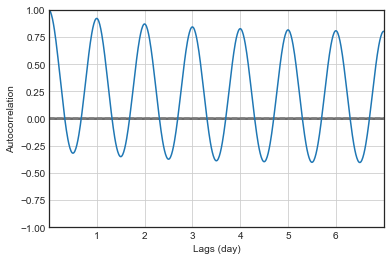
\includegraphics[width=\linewidth]{figures/figure_autocorr_temp.png}
  \caption{Autocorrelation of temperature showing a strong relationship with its daily seasonality (1 interval = 15 minutes)}
  \label{figure_autocorr_temp}
\end{figure}









With these weather variables having a shorter term pattern, these could have situational effects to related or dependent variables whose usual pattern may be disrupted. Thus, we classify these variables as \textit{disruptive variables}. These include wind speed, wind gust, precipitation, and visibility (see Figure \ref{figure_disruptive_var}). Looking at the multicollinearity of these variables (see Figure \ref{figure_weather_corr}), it could be observed most disruptive variables have a strong correlation with precipitation. Particularly, both visibility and wind gust are strongly correlated with precipitation, having a correlation value of -0.787 and 0.600 respectively; and wind gust is strongly correlated with wind speed, with a correlation value of 0.934.


\begin{figure}
  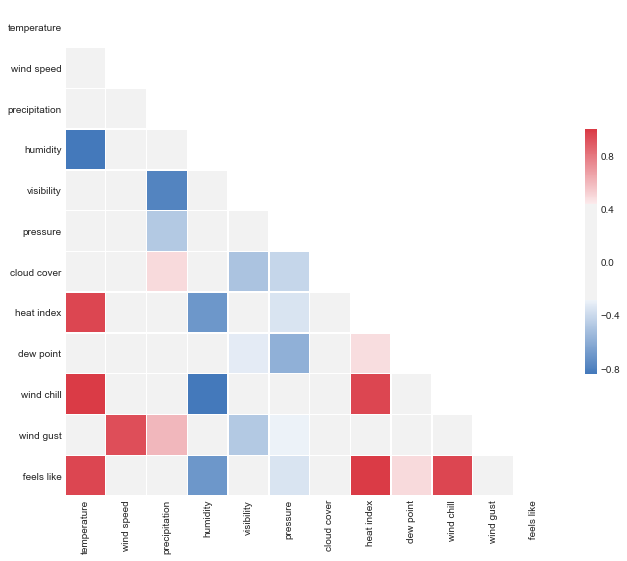
\includegraphics[width=\linewidth]{figures/figure_weather_corr.png}
  \caption{Correlation heatmap of weather variables}
  \label{figure_weather_corr}
\end{figure}








\subsubsection{Trend of Disruptive Variables}

Although these disruptive variables have a shorter term pattern, some still follow certain trends despite being influenced by other disruptive variables. One of which is wind gust (see Figure \ref{figure_windgust}). Similar to non-disruptive variables, wind gust follows a long-term pattern yet is heavily impacted by other disruptive variables, specifically precipitation. It follows the trend of gradually falling until noontime, rising and peaking during the afternoon, and falling at a similar rate during the evening.


\begin{figure}
  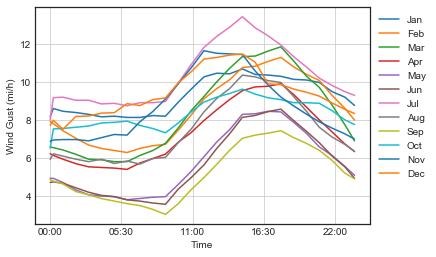
\includegraphics[width=\linewidth]{figures/figure_windgust.png}
  \caption{Daily average of wind gust per month revealing its normal trend despite having a loose daily seasonality}
  \label{figure_windgust}
\end{figure}





In instances where precipitation is abundant, however, there is an immediate effect to its pattern. Figure \ref{figure_precip_temp} and \ref{figure_precip_windgust} shows a comparison of the impact of precipitation to temperature and wind gust in one of the days under Typhoon Egay. It could be observed that the precipitation did not significantly impact the pattern of the temperature. Nevertheless, we could see how it gradually decreased the temperature from its usual pattern in that specific month. Comparing it with wind gust, it could be observed that the effects of precipitation already took an effect on the pattern of wind gust as it starts to build up. Wind speed, being strongly correlated with wind gust, follows this trend as well (see Figure \ref{figure_precip_windspeed}).



% \begin{figure}
% \begin{subfigure}{0.49\textwidth}
% 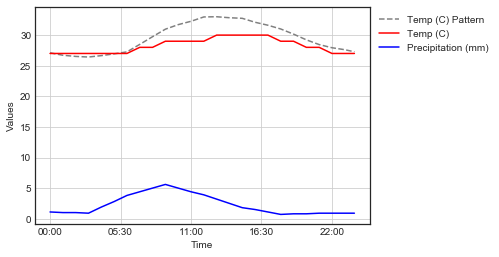
\includegraphics[width=\linewidth]{figures/figure_precip_temp.png}
% \caption{First subfigure} \label{fig:1a}
% \end{subfigure}
% \hspace*{\fill} % separation between the subfigures
% \begin{subfigure}{0.49\textwidth}
% 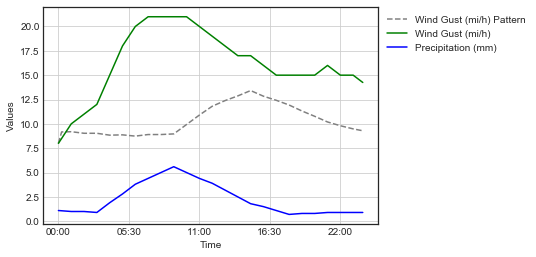
\includegraphics[width=\linewidth]{figures/figure_precip_windgust.png}
% \caption{Second subfigure} \label{fig:1b}
% \end{subfigure}
% \end{subfigure}
% \caption{Comparison of the effects of precipitation to the normal pattern of temperature (a), a non-disruptive variable, and wind gust (b), a disruptive variable} \label{figure_precip_temp_windgust}
% \end{figure}



\begin{figure}
  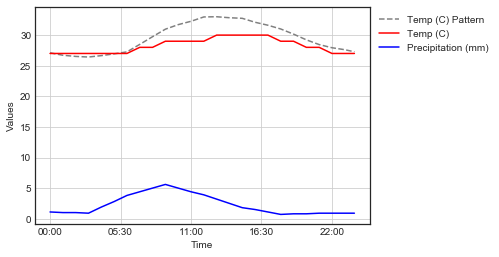
\includegraphics[width=\linewidth]{figures/figure_precip_temp.png}
  \caption{Comparison of the effects of precipitation to the normal pattern of temperature}
  \label{figure_precip_temp}
\end{figure}



\begin{figure}
  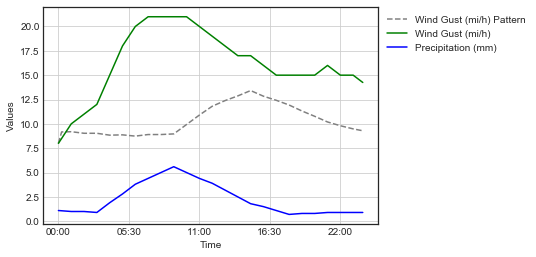
\includegraphics[width=\linewidth]{figures/figure_precip_windgust.png}
  \caption{Comparison of the effects of precipitation to the normal pattern of wind gust}
  \label{figure_precip_windgust}
\end{figure}







\begin{figure}
  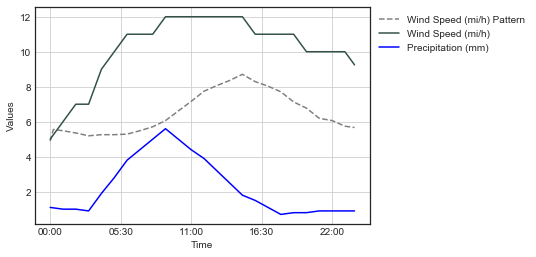
\includegraphics[width=\linewidth]{figures/figure_precip_windspeed.png}
  \caption{Comparison of the effects of precipitation to the normal pattern of wind speed}
  \label{figure_precip_windspeed}
\end{figure}









\begin{figure}
  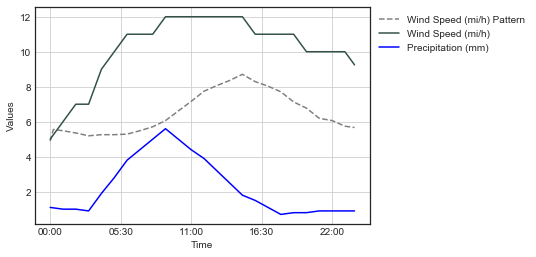
\includegraphics[width=\linewidth]{figures/figure_precip_windspeed.png}
  \caption{Comparison of the effects of precipitation to the normal pattern of wind speed}
  \label{figure_precip_windspeed}
\end{figure}



In a similar way, precipitation also affects other disruptive variables, mainly visibility. Contrary to wind gust and wind speed, visibility does not have a long-term pattern. Rather, it has a strong negative correlation with precipitation, hence its short-term trend is dependent on precipitation instances (see Figure \ref{figure_precip_visibility}).

\begin{figure}
  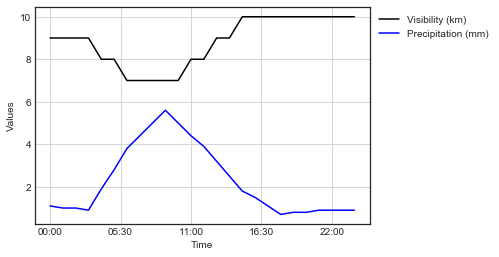
\includegraphics[width=\linewidth]{figures/figure_precip_visibility.png}
  \caption{Negative relationship between visibility and precipitation}
  \label{figure_precip_visibility}
\end{figure}




























\subsection{Traffic Analysis}

\subsubsection{Seasonality}

On an average day, traffic could be linked with the people's daily transportation demand. One example of these is the daily commute of people, attributed to their organizational duties (i.e. 9 to 5 jobs) and academical duties. Built upon these expected demands, the daily seasonality of traffic has been established, following the concept of peak hour. Peak hour refers to the busiest hour where traffic is expected to rapidly rise. In the case of Metro Manila, peak hours are expected to occur from 7 AM to 10 AM, when people leave their home to go to their respective organizations, and 4 PM to 7 PM, when they depart their organizations and return home \cite{metro_manila_peak_hour}.

However, knowing that there are other contributing factors to traffic, its pattern is not consistent despite its daily seasonality. Analyzing its autocorrelation (see Figure \ref{figure_autocorr_traffic_week}), it could be observed that in spite of its daily pattern, its succeeding days are loosely correlated with the present one. Interestingly, though, the traffic pattern of the previous day could also be used as much as the succeeding days or even the week after. Furthermore, compared with the previous days, it could be observed the present traffic is more correlated with its 7-days-ago pattern or its previous week (e.g. relate the present Monday with last week's Monday).
    
    
\begin{figure}
  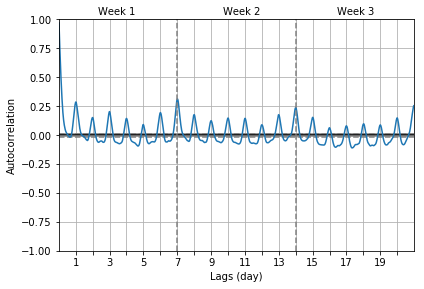
\includegraphics[width=\linewidth]{figures/figure_autocorr_traffic_week.png}
  \caption{Autocorrelation of traffic revealing its daily and weekly seasonality}
  \label{figure_autocorr_traffic_week}
\end{figure}



Viewing its pattern in a longer term, nevertheless, its weekly pattern becomes looser as months go by (see Figure \ref{figure_autocorr_traffic_month}). In other words, it is recommended to expect a certain pattern to last for only four weeks at most. Further examining its seasonality, it could also be observed it does not have a yearly seasonality as well, and its seasonality fades out as time passes by. In simple terms, the traffic pattern in January 2015 is not the same with January 2016. Rather, the traffic pattern in December 2015 is closer to the pattern of January 2016.
    
    
\begin{figure}
  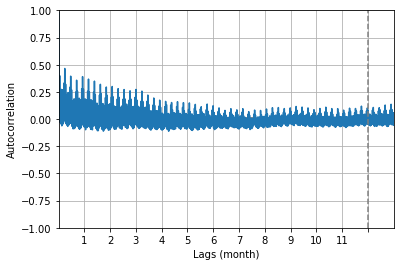
\includegraphics[width=\linewidth]{figures/figure_autocorr_traffic_month.png}
  \caption{Autocorrelation of traffic showing no yearly seasonality}
  \label{figure_autocorr_traffic_month}
\end{figure}


Given these seasonalities, we will explore how traffic changes in its short term and longer term.






\paragraph{Previous Day}

Traffic's daily seasonality could be perceived as causal, such that the traffic of yesterday could be attributed to the traffic of today. For instance, having an intense traffic yesterday morning could be linked with the incoming morning traffic of today. In inheriting the factors of previous days, nonetheless, we also need to take into consideration the concept of working and non-working day.

  A \textit{working day} refers to a day in which people are assigned on duty in an organization \cite{liu2008wdcm}. For most organizations, it is defined to be on weekdays, Mondays to Fridays, while non-working days are on weekends, Saturdays to Sundays. Aside from weekends, though, non-working days also occur during holidays and government-announced class/work suspension. For our analysis, we treated those days as outliers to our data as the traffic pattern for that particular day is irregular compared with the other weekday working day records. These are important to consider as the transportation demand during working days are higher compared with non-working days \cite{traffic_trend}. For example, the transportation demand of Monday is significantly different from Sunday, thus referencing Sunday for the expected pattern of Monday would be erroneous.

  Comparing the average traffic between working days and non-working days in one month, we could see a significant difference in terms of intensity and pattern (see Figure \ref{figure_workingday_comparison}). Majority of intense traffic occurs at working days. Table \ref{table_traffic_cond_workingday} shows that heavy traffic consists 10.584\% of the working day dataset, while only 0.301\% of the non-working day dataset. Moreover, light traffic consists only 51.819\% of the working day dataset while it accounts for 76.973\% of the non-working day dataset. This, in terms of pattern, indicates that non-working day traffic may follow the peak hour-driven traffic pattern. Therefore, in defining a specific peak hour, we must consider non-working days as an inconsistent case if compared with working days.
    

\begin{figure}
  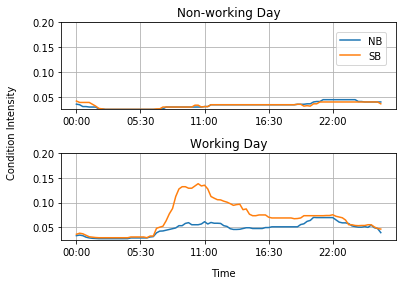
\includegraphics[width=\linewidth]{figures/figure_workingday_comparison.png}
  \caption{Comparison of traffic condition intensity between non-working and working revealing the lack of intense traffic for non-working days}
  \label{figure_workingday_comparison}
\end{figure}

\begin{table}[t]

\centering
\caption{Comparison of traffic condition distribution between working and non-working}
\label{table_traffic_cond_workingday}

\begin{tabular}{|l|r|r|}
\hline
\textbf{Traffic Condition} & \textbf{Working Day} & \textbf{Non-working Day} \\ \hline
L                          & 51.876\%             & 76.973\%                 \\ \hline
ML                         & 4.051\%              & 3.085\%                  \\ \hline
M                          & 31.917\%             & 19.461\%                 \\ \hline
MH                         & 1.573\%              & 0.180\%                  \\ \hline
H                          & 10.584\%             & 0.301\%                  \\ \hline
\end{tabular}
\end{table}


\paragraph{Previous Week}

Traffic could also be related to its week-ago traffic pattern. There has been a concept known as Monday rush hour and Friday rush hour where traffic is expected to increase in the morning and at night respectively. Similar to the previous day approach, we also need to consider working days, but to a lesser degree. Instead, we would only take into account the holidays and suspensions which we will similarly treat as outliers in our reference. To support its weekly seasonality, in \figref{figure_traffic_day_vs_week}, it could be observed how closer the traffic pattern is with its one-week-ago pattern compared with its two-day-ago pattern.



\subsubsection{Connected Road Segments}

After analyzing the pattern of a road segment with its own pattern, we now analyze it as a part of a road. Aside from itself, its traffic could also be linked with its relationship with its connected road segments. Exploring the working day traffic of all road segments in Roxas Boulevard, it could be observed that there is an intensity relationship between these road segments. The intense traffic of Pablo Ocampo is carried over to Quirino in a similar intensity yet continuously decays as we go further to Anda Circle. Likewise, the intensity of the traffic of Blumentritt rises as we approach Antipolo then decays as we go further to Lerma.


\subsubsection{Rolling and Expanding Features}

The data only describes the traffic condition per timestep and the seasonality of traffic. Although traffic has pattern, there are instances when a certain disruption in traffic may cause congestion build up. Therefore, considering how the past traffic conditions may affect the current traffic condition can be considered as a factor for predicting traffic. Although the data from the previous timestep can be used as a reference in predicting the current traffic condition, the change in traffic in a 15-minute timeframe may not be significant. As seen in \figref{figure_autocorr_traffic_workingdays}, autocorrelation reveals that a traffic condition is highly likely to reoccur every 15 minutes with a correlation value of 0.9918. In other words, the traffic condition of the previous time step is highly likely to be the traffic condition of the current time step. However, this does not capture the effects of sudden outliers to the build up or decay of traffic. Thus, it does not fully describe how the past traffic conditions might affect the current traffic condition. 

\begin{figure}
  \centering
  \captionsetup{justification=centering}
  \scalebox{.80}{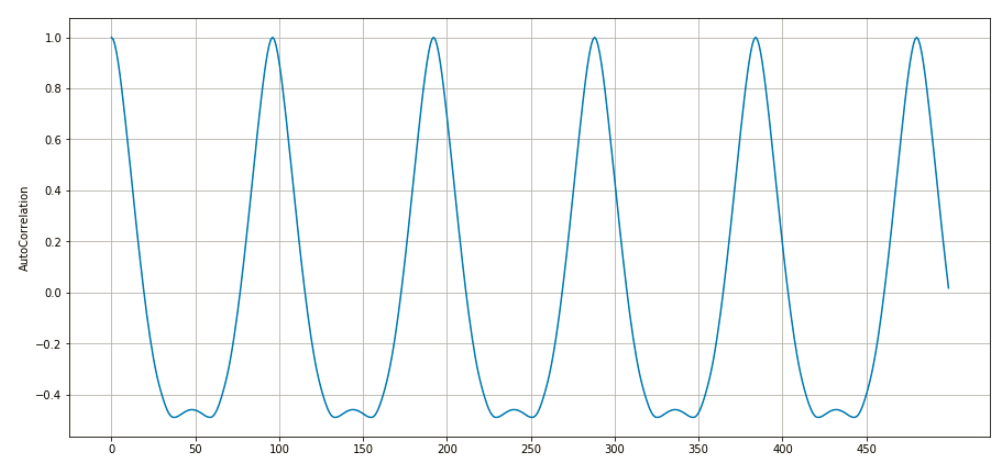
\includegraphics{autocorr_whyRE.PNG}}
  \caption{Autocorrelation of traffic for working days}
  \label{figure_autocorr_traffic_workingdays}
\end{figure}

Generating rolling and expanding features based on a specific window size gives a bigger look as to what the current traffic might be based from the previous traffic conditions. Rolling and expanding traffic features such as the mean, the minimum, and the maximum with window size  4, 8, 24, 48, and 96 were generated from the original traffic data. To summarize the possible effects of sudden changes in traffic, the mean of the past traffic conditions based on a window size was generated. Figure \ref{figure_stdev_traffic} shows the standard deviation values of traffic for every window size. Standard deviation shows the variability or the distance of the data from the mean. From this, it can be observed that there is a logarithmic pattern in the growth of the standard deviation as the window size increases. The low standard deviation of smaller window sizes signifies that there is only a little to no change in traffic condition within that time frame. Meanwhile, large window sizes like window 96 which yield a relatively larger standard deviation value of 0.03531 than of window 4, implies that the traffic conditions in a 1-day time frame are more varied or are more widely spread. With small window sizes, the values generated captures less of the trifle changes in traffic and gets more affected by outlier values which then results in a more generic information. However, as the window size increases, the effect of outlier values also get more neutralized because of the number of data considered, giving a broader summary of the past traffic. 

\begin{figure}
  \centering
  \captionsetup{justification=centering}
  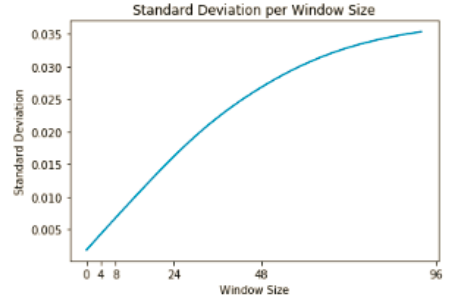
\includegraphics{stDev.PNG}
  \caption{Standard deviation per window size of northbound traffic in Bluementritt for wet season}
  \label{figure_stdev_traffic}
\end{figure}


Unlike the rolling mean, the expanding mean bases its computations on a growing window size and goes back to window size 1 when it reaches a specific maximum window size. This lessens the probability of the outliers getting majorly and consistently neutralized since it always goes back to the original traffic condition from the previous timestep. Thus, revealing less generalized details.

The minimum and maximum features, on the other hand, reveals the range of the dataset. Being sensitive to outliers, they provide outlier detection when compared to the average value of that specific set of data. A big difference between the values of the minimum and the maximum signifies a large progression in traffic condition. Although as the window size used gets bigger, it becomes harder to determine whether the sudden change in traffic condition occurred just a few timesteps before or if it is because of a farther instance which may have less to no effect to the current traffic condition. 

Figures \ref{fig:EspanaRE} and \ref{fig:RoxasRE} show the average correlation of northbound road segments of Espana and southbound road segments of Roxas Boulevard per window size in relation to traffic for both rolling and expanding windows. On average, the original traffic has a strong relationship with rolling features having small window size, specifically window 4 with a correlation value of 0.7501. It is noticeable, however, that the strength of the relationship dwindles down as the window size increases. This reveals that although having a bigger window size means being able to capture various changes in traffic condition, it does not give importance to the most recent traffic conditions. Big changes in traffic conditions that occurred way back and may not have any effect on the current traffic are being considered. Thus, causing its misalignment to the original data. 

In the case of expanding windows, the strength of the relationship to the original traffic also decreases as the window size increases, albeit not so much as the rolling mean do. Looking into both graphs, the strength of the relationship given by window 4 for both rolling and expanding is distinctly stronger compared to the ones with larger window size. This might be because as mentioned earlier, traffic does not usually change significantly within a small window. Furthermore, a smaller window size means that its frequency of reverting back to the original value, making its generated value more accurate. Meanwhile, the farther from the past that it considers, the less it captures changes in traffic. This is shown in Figures \ref{fig:bluementritt_rolling} and \ref{fig:bluementritt_expanding}, where rolling and expanding at window 96 generalizes the high condition intensities into information that is no longer close to reality. Furthermore, the plodding decrease of correlation strength in expanding features as compared to rolling features is caused by limiting the number of windows that the feature grows to and considers and the restarting of its window size. Not limiting the window size growth of expanding features would produce values that are very far away from reality because it would consider every data from the previous days. It would contain values that consider data that are not relevant in predicting the future traffic.



\begin{figure}
    \centering
      \captionsetup{justification=centering}
    \subfloat[EspanaRE]{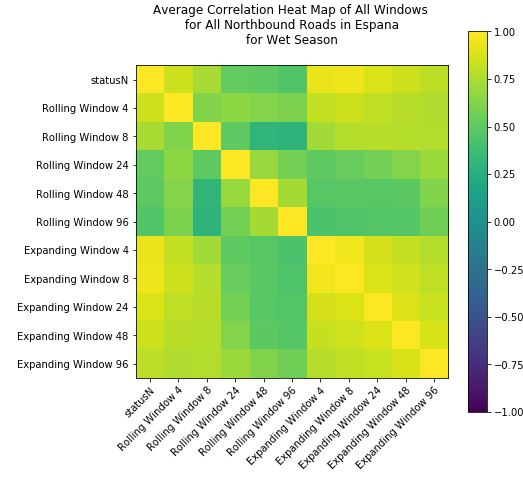
\includegraphics[width=0.5\textwidth]{figures/heatmap_espana.JPG}\label{fig:EspanaRE}}
    \hfill
    \subfloat[RoxasRE]{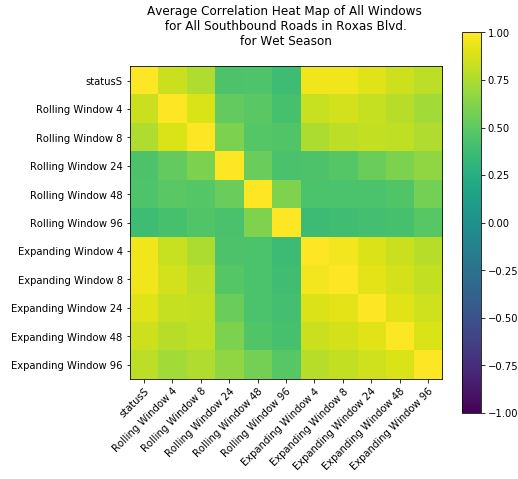
\includegraphics[width=0.5\textwidth]{figures/heatmap_roxas.JPG}\label{fig:RoxasRE}}
    \caption{Average Correlation of Rolling and Expanding Features for Espana and Roxas Blvd.}
\end{figure}

\begin{figure}
    \centering
      \captionsetup{justification=centering}
    \subfloat[Original vs. Rolling]{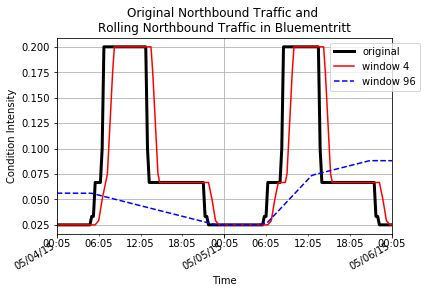
\includegraphics[width=0.5\textwidth]{bluementritt_rolling.png}\label{fig:bluementritt_rolling}}
    \hfill
    \subfloat[Original vs. Expanding]{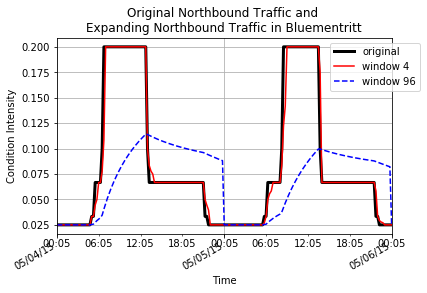
\includegraphics[width=0.5\textwidth]{bluementritt_expanding.png}\label{fig:bluementritt_expanding}}
    \caption{Comparison of Rolling and Expanding windows 4 and 96 to original Southbound traffic in Bluementritt}
\end{figure}


\subsection{Relationship of Weather to Traffic}
\subsubsection{Daytime and Nighttime}
\subsubsection{Time of Day}


\subsection{Effects of Weather to Traffic}
\subsubsection{Precipitation}
\subsubsection{Season by Precipitation Rate}
\subsubsection{Weather Disruption}



\section{Prediction Model Analysis}
To test and evaluate the performance of the model in the presence of weather changes, two datasets for both dry (January to April, and November to December) and wet season (May to October) were used. Traffic and weather data were provided by MMDA and WWO, respectively. The models were evaluated using root mean squared error (RMSE) and mean absolute error (MAE). 


\subsection{Traffic-Only Model}
To evaluate the performance of TOM, and the effectiveness of engineering features for traffic, combination of features were used and compared for all road segments for both wet and dry season. These features include temporal information about the current traffic (i.e. month, day, hour, minute, and day of the week), past traffic of 96 intervals in the past or traffic the day before, flags for work days and peak hours, and rolling and expanding window of traffic 15 minutes in the past. Based on earlier discussions, rolling and expanding windows are not correlated with each other. Thus, rolling and expanding window features are used together in the model. In further figures in discussing the Traffic-Only Model, the different feature combinations are denoted as the following:

\begin{enumerate}
\item \textit{OT} - Features that only consist of the past traffic a day before the current;
\item \textit{OTWP} - Features including past traffic a day before the current, and flags on the workday and peak hour, and;
\item \textit{WPRE}- Features including OTWP, plus the addition of rolling and expanding features of the traffic 15 minute in the past of the current. In subsequent discussions, any number following this notion pertains to the window size of both the rolling and expanding features (e.g. WPRE 4 pertains to the features that include rolling and expanding features of window size 4).
\end{enumerate}

As seen in Figure \ref{fig:tom_diff_feat_combi} the inclusion of the information about working days and peak hours for all road segments improved the performance of the model by only 22\% having originally an RMSE of 0.167 which improved to 0.113. As discussed earlier on the trend and patterns of traffic, though there is a difference between the trends of working days and non-working days, moderate traffic is most frequent in both trends in the majority of the road segments, This implies that the mean traffic intensity for both working and non-working days are similar. This similarity attributes to the small improvement in the prediction. Furthermore, including rolling and expanding window features for traffic significantly improved the prediction by around 53\%, from having an RMSE of 0.129 to 0.061 after adding the said features. Rolling window features present a generalized information regarding the trend of the immediate past traffic. As discussed earlier, average traffic does not change significantly within a small window.   

\begin{figure}
  \centering
  \captionsetup{justification=centering}
  \scalebox{0.6}{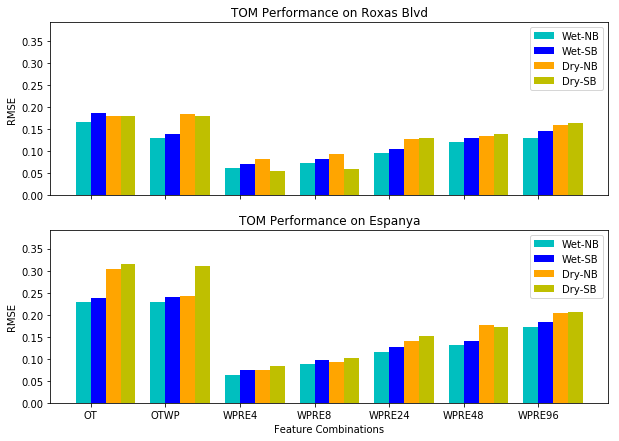
\includegraphics{tom_diff_feat_combi.png}}
  \caption{Comparison between performance of TOM on Roxas Boulevard and Espana using different feature combinations}
  \label{fig:tom_diff_feat_combi}
\end{figure}


To evaluate if the model can successfully identify the trends present for each road segment, and its ability to predict its traffic, the performance of the model using OTWP or Original Traffic with the addition of work day and peak hours was observed. Results of this evaluation are illustrated in Figure \ref{fig:tom_feat_combi_road}. It is noticeable that the model predicted the southbound traffic of Espanya during the wet season quite well, having a mean RMSE of 0.095 compared to the other. However, this is because of the diversity of the southbound traffic of Espanya during the wet season, having a Moderate traffic congestion majority of the time. Given only data of the previous day’s traffic, and information on work day and peak hours, the model cannot easily model the sudden peaks and traffic reports on Heavy traffic. Additionally, given the percentage of the report on Heavy traffic congestion of the data, having only 10.584\% during the working days, and 0.301\% during the non-working days, the model lacks knowledge on modeling expected heavy traffic. 

\begin{figure}
  \centering
  \captionsetup{justification=centering}
  \scalebox{0.6}{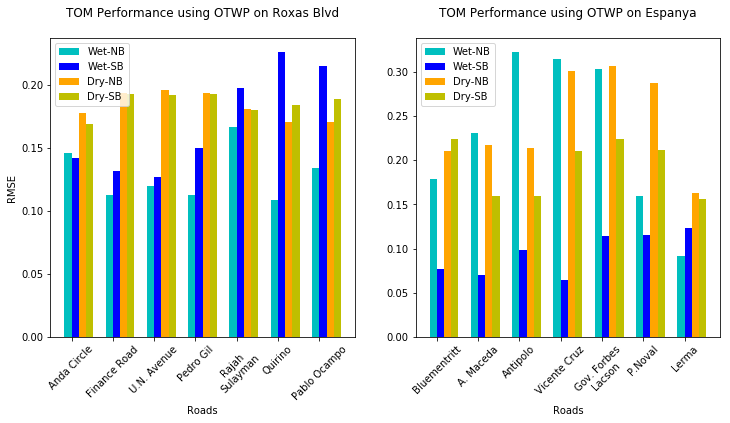
\includegraphics{tom_feat_combi_road.png}}
  \caption{Performance of TOM on Roxas Boulevard and Espanya using OTWP traffic feature combination}
  \label{fig:tom_feat_combi_road}
\end{figure}



\subsection{Weather-Only Model}
In earlier discussions regarding the relationship between weather variables with traffic, most weather variables had a weak relationship with traffic. To further evaluate this, the Weather Only Model was tested using three different combinations of weather variables which are:

\begin{enumerate}
\item Original Weather (OW) - all weather variables
\item All Correlated Weather (ACW) - all weather variables that have correlation between 0.1 to 0.3
\item Correlated Weather (CW) - all correlated weather variables excluding the redundant ones
\end{enumerate}

Given the weak relationship between weather variables with traffic, the model could only predict traffic about 80 to 84\% after using weather variables for input as compared to using past traffic that can predict traffic by 90\%. Furthermore, the model’s performance did not improve significantly with different combinations (see Figure \ref{fig:wom_diff_feat_combi}) of weather variables having changes in error ranging from only 0.001 to 0.003. 

\begin{figure}
  \centering
  \captionsetup{justification=centering}
  \scalebox{0.7}{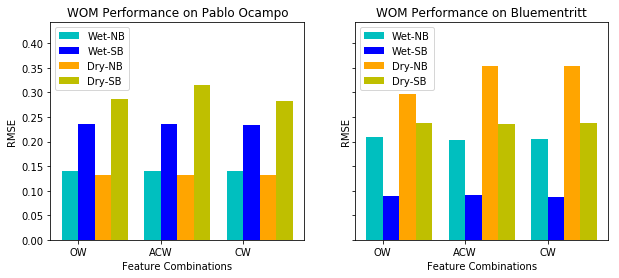
\includegraphics{wom_diff_feat_combi.png}}
  \caption{Performance of WOM on Pablo Ocampo and Bluementritt using weather feature combinations}
  \label{fig:wom_diff_feat_combi}
\end{figure}

Illustrated in Figure \ref{fig:wom_diff_feat_combi} is the performance of the weather only model using the three feature combinations for the road segment of Pablo Ocampo and Blumentritt. As seen in the figure, the model predicted the northbound traffic in Pablo Ocampo better than the southbound traffic. According to data analysis performed above, the northbound traffic in Pablo Ocampo has more reports on heavy traffic than the southbound. Likewise, the model predicted the southbound of Bluementritt better than the northbound. However, in Pablo Ocampo, the model performed better using the northbound traffic for both dry and wet season, as for Bluementritt, the model performed better when using the wet season dataset, for both northbound and southbound. During the wet season of 2015, the traffic in Bluementritt was less diverse having a mean traffic for southbound of 0.187 and mean traffic for northbound of 0.208, both values close near the value for moderate traffic of 0.238. This means that traffic congestion level in Bluementritt for both southbound and northbound during the wet season is mostly moderate. This is further supported by evaluating the model’s performance with other connected road segments as seen in Figure \ref{fig:wom_feat_combi_roads} which shows the performance of the weather only model using all weather features for all road segments. Other road segments follow the said behavior.

\begin{figure}
  \centering
  \captionsetup{justification=centering}
  \scalebox{0.6}{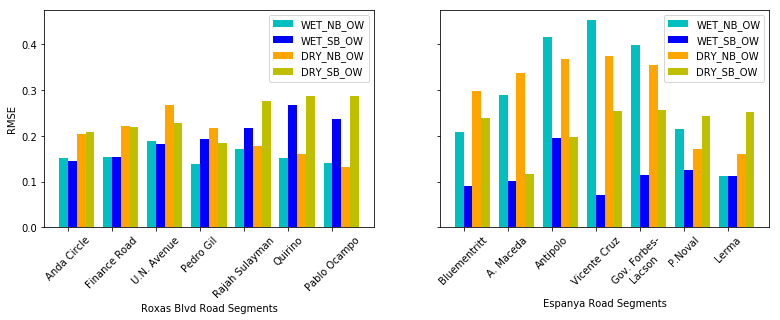
\includegraphics{wom_feat_combi_roads.png}}
  \caption{Performance of WOM using OW weather feature combination for all road segments}
  \label{fig:wom_feat_combi_roads}
\end{figure}



\subsection{Fusion Analysis}
Different fusion techniques and approaches were used and evaluated. The performance of fusing in the feature and decision level was first evaluated. Then, the performance of fusing in the decision level using a number of fusion algorithms was observed. Table \ref{table:fusion_results} displays the different performances in different fusion approaches and techniques. 

\begin{table}[]
\begin{tabular}{|l|r|r|r|r|r|r|}
\hline
\multirow{2}{*}{\textbf{Fusion Techniques}} & \multicolumn{2}{c|}{\textbf{OTWP + OW}}                                & \multicolumn{2}{c|}{\textbf{WPRE 4 + OW}}                              & \multicolumn{2}{l|}{\textbf{WPRE 96 + OW}}                             \\ \cline{2-7} 
                                            & \multicolumn{1}{c|}{\textbf{RMSE}} & \multicolumn{1}{l|}{\textbf{MAE}} & \multicolumn{1}{c|}{\textbf{RMSE}} & \multicolumn{1}{l|}{\textbf{MAE}} & \multicolumn{1}{l|}{\textbf{RMSE}} & \multicolumn{1}{l|}{\textbf{MAE}} \\ \hline
\textbf{DBN Feature Fusion}                 & 0.262                              & 0.156                             & 0.079                              & 0.030                             & 0.219                              & 0.122                             \\ \hline
\textbf{DBN Decision Fusion}                & 0.244                              & 0.173                             & \textbf{0.070}                     & \textbf{0.025}                    & 0.144                              & 0.079                             \\ \hline
\textbf{RNN Decision Fusion}                & \textbf{0.068}                     & \textbf{0.054}                    & 0.171                              & 0.131                             & \textbf{0.103}                     & \textbf{0.085}                    \\ \hline
\textbf{WA Decision Fusion}                 & 1.087                              & 1.048                             & 0.497                              & 0.457                             & 0.727                              & 0.700                             \\ \hline
\end{tabular}
\caption{Performance of different fusion techniques in different feature combinations}
\label{table:fusion_results}
\end{table}

Although the results display a difference between the performance of fusing at the feature level to decision level, the model only improved by 6.87\% in fusing at the decision level. 

The performance of WA in fusing data with the least-square estimate was greatly outshone by the two neural network fusion algorithms. Fusing with WA gained an RMSE of 1.087 and an MAE of 1.048, having a significant difference in error of 1.019 to 0.843 as compared to the other fusion algorithms. The algorithm for weighted average for fusing the predictions made used of least square estimate method to determine the fusion’s weights. Least-square estimate is defined as the minimum of the sum of squared residuals, or the difference between the actual and the predicted. This method is most useful when used in data which are more linear, where the pattern of the data can be extracted through simply just getting the residual, the slope of the line, and the coefficients of the input. This method of pattern extraction is called regression. The coefficients of the input generated after regression analysis are used as weights in the study’s Weighted Average algorithm. Given the behavior of the algorithm, it fails to extract patterns from the non-linear data. For the subsequent experiment and analysis, WA is disregarded. 

RNN outperforms DBN, and other fusion algorithms by 74\%. RNN is implemented as an LSTM, or a long short-term memory, compared to DBN which is implemented as a regressor and a classifier. Because of RNN’s power of long short-term memory, it can use their internal memory to process a sequence of inputs, successfully extracting ordered patterns. 

In evaluating the effect of the inclusion of weather as a factor in predicting traffic, the performance of the Traffic-Only Model, the model that can predict traffic using only the immediate past traffic, is compared with the performance of the fusion for all techniques. Results are illustrated in Figure \ref{fig:dbn_comp_pocampo}, which displays that the prediction improves after using weather as a factor. Though the improvement in performance is only 14\%, the improvement was consistent for different combinations of features. A contributor to the low improvement is the number of observations that weather is present when traffic least expected. For example, according to the weather data, heavy rainfall was present during September 11-12 of 2015, a Friday and a Saturday, when traffic is least expected. Additionally, rain started to fall at night of September 11, extending until the early morning of September 12. There were few records that successfully capture the contributing factor of weather towards traffic given the time periods disrupting weather variables were often present. For visualization purposes, the predicted traffic is illustrated in Figure \ref{fig:final_prediction}

\begin{figure}
  \centering
  \captionsetup{justification=centering}
  \scalebox{0.35}{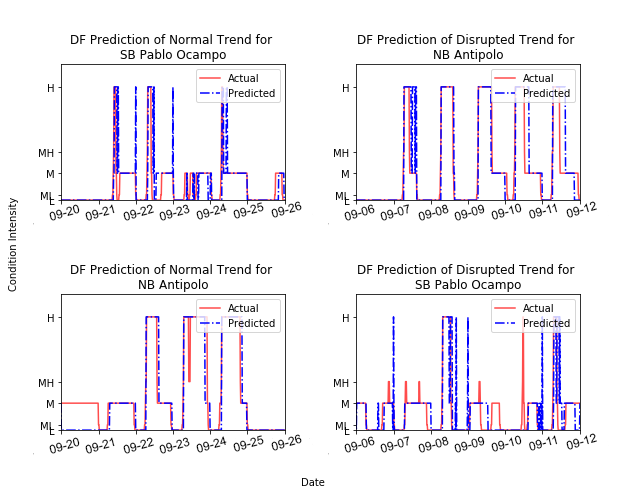
\includegraphics{final_prediction.png}}
  \caption{Final Prediction of Southbound of Pablo Ocampo for the Month of September}
  \label{fig:final_prediction}
\end{figure}


\begin{figure}
  \centering
  \captionsetup{justification=centering}
  \scalebox{0.7}{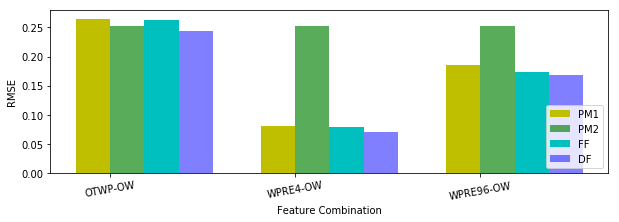
\includegraphics{dbn_comp_pocampo.png}}
  \caption{Comparison of DBN model in predicting the southbound of Pablo Ocampo for the wet season}
  \label{fig:dbn_comp_pocampo}
\end{figure}



\subsection{Sensitivity Analysis}

\subsubsection{Traffic-Only Model}

First, the sensitivity of the predictions models with changing input variables was evaluated. In evaluating TOM, the different input variables were removed per experiment to see the effect of its inclusion. The combination of input variables were done in the feature combination in earlier evaluations of the model (e.g. OTWP, OT, WPRE, OW, etc). For example, variables of the OTWP feature combination were tinkered. Then, the variables of OT combination were evaluated, and so on. The temporal information was the first set of features of the combination that were removed one-by-one, then information on past traffic. The base model, with all the features including temporal and past traffic, was compared with the model with the removed variables (with or without temporal information or past traffic), and its change in performance was evaluated. The changes in performance illustrates the sensitivity of the model. 

\begin{figure}
  \centering
  \captionsetup{justification=centering}
  \scalebox{0.6}{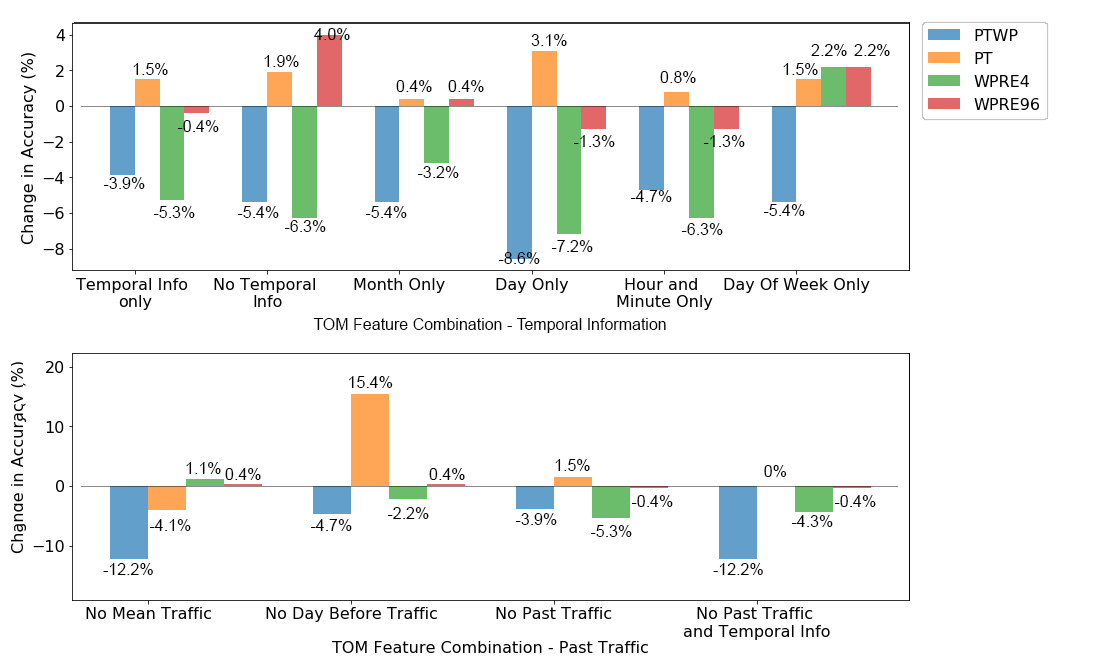
\includegraphics{TOM_sensitivity.png}}
  \caption{Sensitivity of TOM with different feature combinations}
  \label{fig:TOM_sensitivity}
\end{figure}


Evaluation on the sensitivity of TOM is illustrated in \ref{fig:TOM_sensitivity}. It has been discussed in the early sections in evaluating TOM that the inclusion of Work day, and Peak hour variables result to a 22\% improvement in performance. The removal of temporal information decreased the performance from 3.9 to 8.6\% when used with work day and peak hour. Not one temporal information variable increase the accuracy of the base which used all the temporal information, and all past traffic features. However, without the work day and peak hour, removal of the temporal information seems to have increase the performance, but only by 1 to 3\%. Results show that temporal information, when used with working day and peak hour variables without past traffic information, decreases the performance by 4\%. Moreover, each variable excluding the $Day$ variable are independent of each other as seen by the change of accuracy when using only Month, Hour and minute, or day of week. Using the day variable without the support of other temporal information have decreased the performance by 8.6\%. Results show that traffic does not have any pattern with the $Day$ variable. As for the use of temporal information without working day and peak hour, the model performed better. Working day and peak hour variables show a generalized information of traffic at a specific time period. Without this information, the temporal information instead gives information on the traffic such as what hours, or day of week are there heavy traffic condition intensity. 

Looking into the effect of the past traffic feature when used with the work day and peak hour, using either the mean of traffic 2 weeks ago, and a day before did not affect the performance, only having differences of 0.03\%. However, There are significant change when work day and peak hours are not used. In using only the traffic a day before, the performance decreased by 4.1\%. Using the traffic of 2 weeks ago significantly increased the performance by 15.4\%. Results show that the base model for OT that used all the past traffic features of a day and 2 weeks ago and all temporal information without workday and peak hour, gets most of its prediction bases from the general traffic 2 weeks ago. This shows that this variable have great importance in predicting traffic, when working day and peak hours are not used.  

\subsubsection{Decision Fusion Model}

\begin{figure}
  \centering
  \captionsetup{justification=centering}
  \scalebox{0.6}{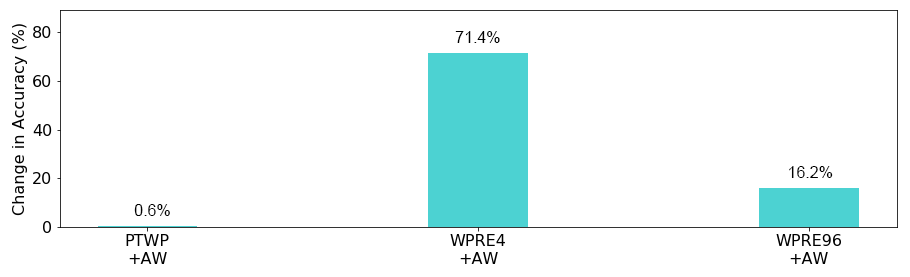
\includegraphics{pm1-pm2-df-changes.png}}
  \caption{Change in performance in different feature combinations}
  \label{fig:pm1-pm2-df-changes}
\end{figure}


The base model for evaluating the fusion between using the different prediction models, and fusion models is the Traffic-Only for OTWP feature combination. As discussed in the Fusion Analysis, considering the weather prediction in fusing at decision level resulted in a 14\% improvement in performance. However, in evaluating the performance of the weather in predicting traffic, weather only contributed about 27\% of the prediction. As mentioned in earlier discussions, traffic data mostly comprises of Moderate traffic condition intensity reports. Additionally, periods where there is a disruption in weather in which traffic is expected lies in weekends, when traffic is least expected. The data does not completely represent the relationship between weather and traffic, thus resulting to the small weight in prediction. 
